\subsection{Router}\label{sec:router}

The preceding sections introduced the eight specialist agents of the PropDesk scenario, each with its own instructions, domain knowledge, and, in production, its own tools and data access. The router assigns every incoming broker query to exactly one of these agents. Queries that fit no specialist domain fall by design to GeneralPurpose, keeping the problem a closed eight-class classification. Misclassification is expensive, since a misrouted specialist returns an answer useless to the advisor. The router must produce a score for each agent and select the highest, so the central design question is how these eight scores are computed. Candidate mechanisms range from asking a model to state its own confidence to measuring semantic similarity, and they differ considerably along the success criteria the project scope fixed before the first sprint, namely accuracy, latency, and cost (see \cref{sec:introduction}). A mechanism that maximizes one dimension while ignoring the other two was ruled out.

\subsubsection{Routing Mechanisms Considered}\label{sec:router-mechanisms}

The candidate mechanisms draw on two largely separate research strands. One strand studies how language models assess their own reliability \autocite{kadavath2022,tian2023,xiong2024}. The other studies how queries are routed between models, typically with dedicated classifiers trained on preference or performance data \autocite{ong2024,chen2023}. Using a model's own confidence signal as routing criterion sits between these strands and is comparatively unexplored, so no established default existed. We therefore analyzed four candidates.

Verbalized confidence asks the routing model to state a confidence value per agent in plain text. It requires no infrastructure change, and our initial system routed exclusively this way, making it the natural baseline. The literature, however, speaks against it as a permanent solution. Models tuned with human feedback verbalize systematically overconfident scores \autocite{tian2023}, and the stated values fluctuate with minor changes in prompt wording \autocite{xiong2024}. A router built on this signal inherits both defects, and our own early tests pointed in the same direction.

Self-consistency samples the router several times at nonzero temperature and scores each agent by the fraction of samples that select it \autocite{wang2023}. The approach is robust and needs no model internals, but multiplies cost and latency by the sample count. Its value also lies in aggregating sampled reasoning chains. A routing decision, however, is a single token, and sampling one token merely approximates the distribution that a single forward pass with token probabilities provides exactly.

Log probabilities read that distribution directly. The routing prompt fixes the answer format to a single token identifying one agent, and the probabilities of the eight admissible tokens are taken from the model's prediction layer instead of its generated text. The result is deterministic, arrives in one forward pass, and contains the full distribution over all eight candidates. Signals read from model internals are also those for which \textcite{kadavath2022} report the most reliable calibration. The drawback is technical, since the serving stack must expose token-level log probabilities.

Embedding similarity involves no language model reasoning at all. The query is embedded once and compared to reference material per agent, at a cost several orders of magnitude below an LLM call. This simplicity is also its weakness. A purely semantic match resolves queries whose intent is semantically unambiguous but fails where the surface form resembles the wrong agent.

\Cref{tbl:mechanisms} compares the four options against the three criteria. None satisfies all of them alone. Verbalized confidence and self-consistency are dominated, while embedding similarity and log probabilities are complementary, which led to combining the latter two in a cascade in the spirit of FrugalGPT, where a cheap mechanism answers what it can answer safely and only the remainder passes to an expensive one \autocite{chen2023}. Stage 1 routes by semantic recognition, Stage 2 deliberates over the cases recognition cannot settle (see \cref{fig:pipeline}), following the dual-process idea of \textcite{kahneman2011}. The verbalized-only router remained in place as the comparison point for \cref{sec:empirical-evaluation}.

\begin{longtable}[]{@{}
  >{\raggedright\arraybackslash}p{(\linewidth - 8\tabcolsep) * \real{0.2442}}
  >{\raggedright\arraybackslash}p{(\linewidth - 8\tabcolsep) * \real{0.2674}}
  >{\raggedright\arraybackslash}p{(\linewidth - 8\tabcolsep) * \real{0.1279}}
  >{\raggedright\arraybackslash}p{(\linewidth - 8\tabcolsep) * \real{0.1279}}
  >{\raggedright\arraybackslash}p{(\linewidth - 8\tabcolsep) * \real{0.2326}}@{}}
\caption{The four candidate mechanisms against the success criteria of \cref{sec:introduction} (own illustration).}\label{tbl:mechanisms}\tabularnewline
\toprule\noalign{}
\begin{minipage}[b]{\linewidth}\raggedright
Mechanism
\end{minipage} & \begin{minipage}[b]{\linewidth}\raggedright
Score quality
\end{minipage} & \begin{minipage}[b]{\linewidth}\raggedright
Latency
\end{minipage} & \begin{minipage}[b]{\linewidth}\raggedright
Cost
\end{minipage} & \begin{minipage}[b]{\linewidth}\raggedright
Key limitation
\end{minipage} \\
\midrule\noalign{}
\endfirsthead
\toprule\noalign{}
\begin{minipage}[b]{\linewidth}\raggedright
Mechanism
\end{minipage} & \begin{minipage}[b]{\linewidth}\raggedright
Score quality
\end{minipage} & \begin{minipage}[b]{\linewidth}\raggedright
Latency
\end{minipage} & \begin{minipage}[b]{\linewidth}\raggedright
Cost
\end{minipage} & \begin{minipage}[b]{\linewidth}\raggedright
Key limitation
\end{minipage} \\
\midrule\noalign{}
\endhead
\bottomrule\noalign{}
\endlastfoot
Verbalized confidence & low, overconfident & 1 LLM call & 1 LLM call & unreliable signal \\
Self-consistency & medium, robust & k LLM calls & k LLM calls & k-fold overhead \\
Log probabilities & high, full distribution & 1 LLM call & 1 LLM call & needs logprob access \\
Embedding similarity & high if unambiguous & ms & negligible & fails on ambiguity \\
\end{longtable}

\begin{figure}
\centering
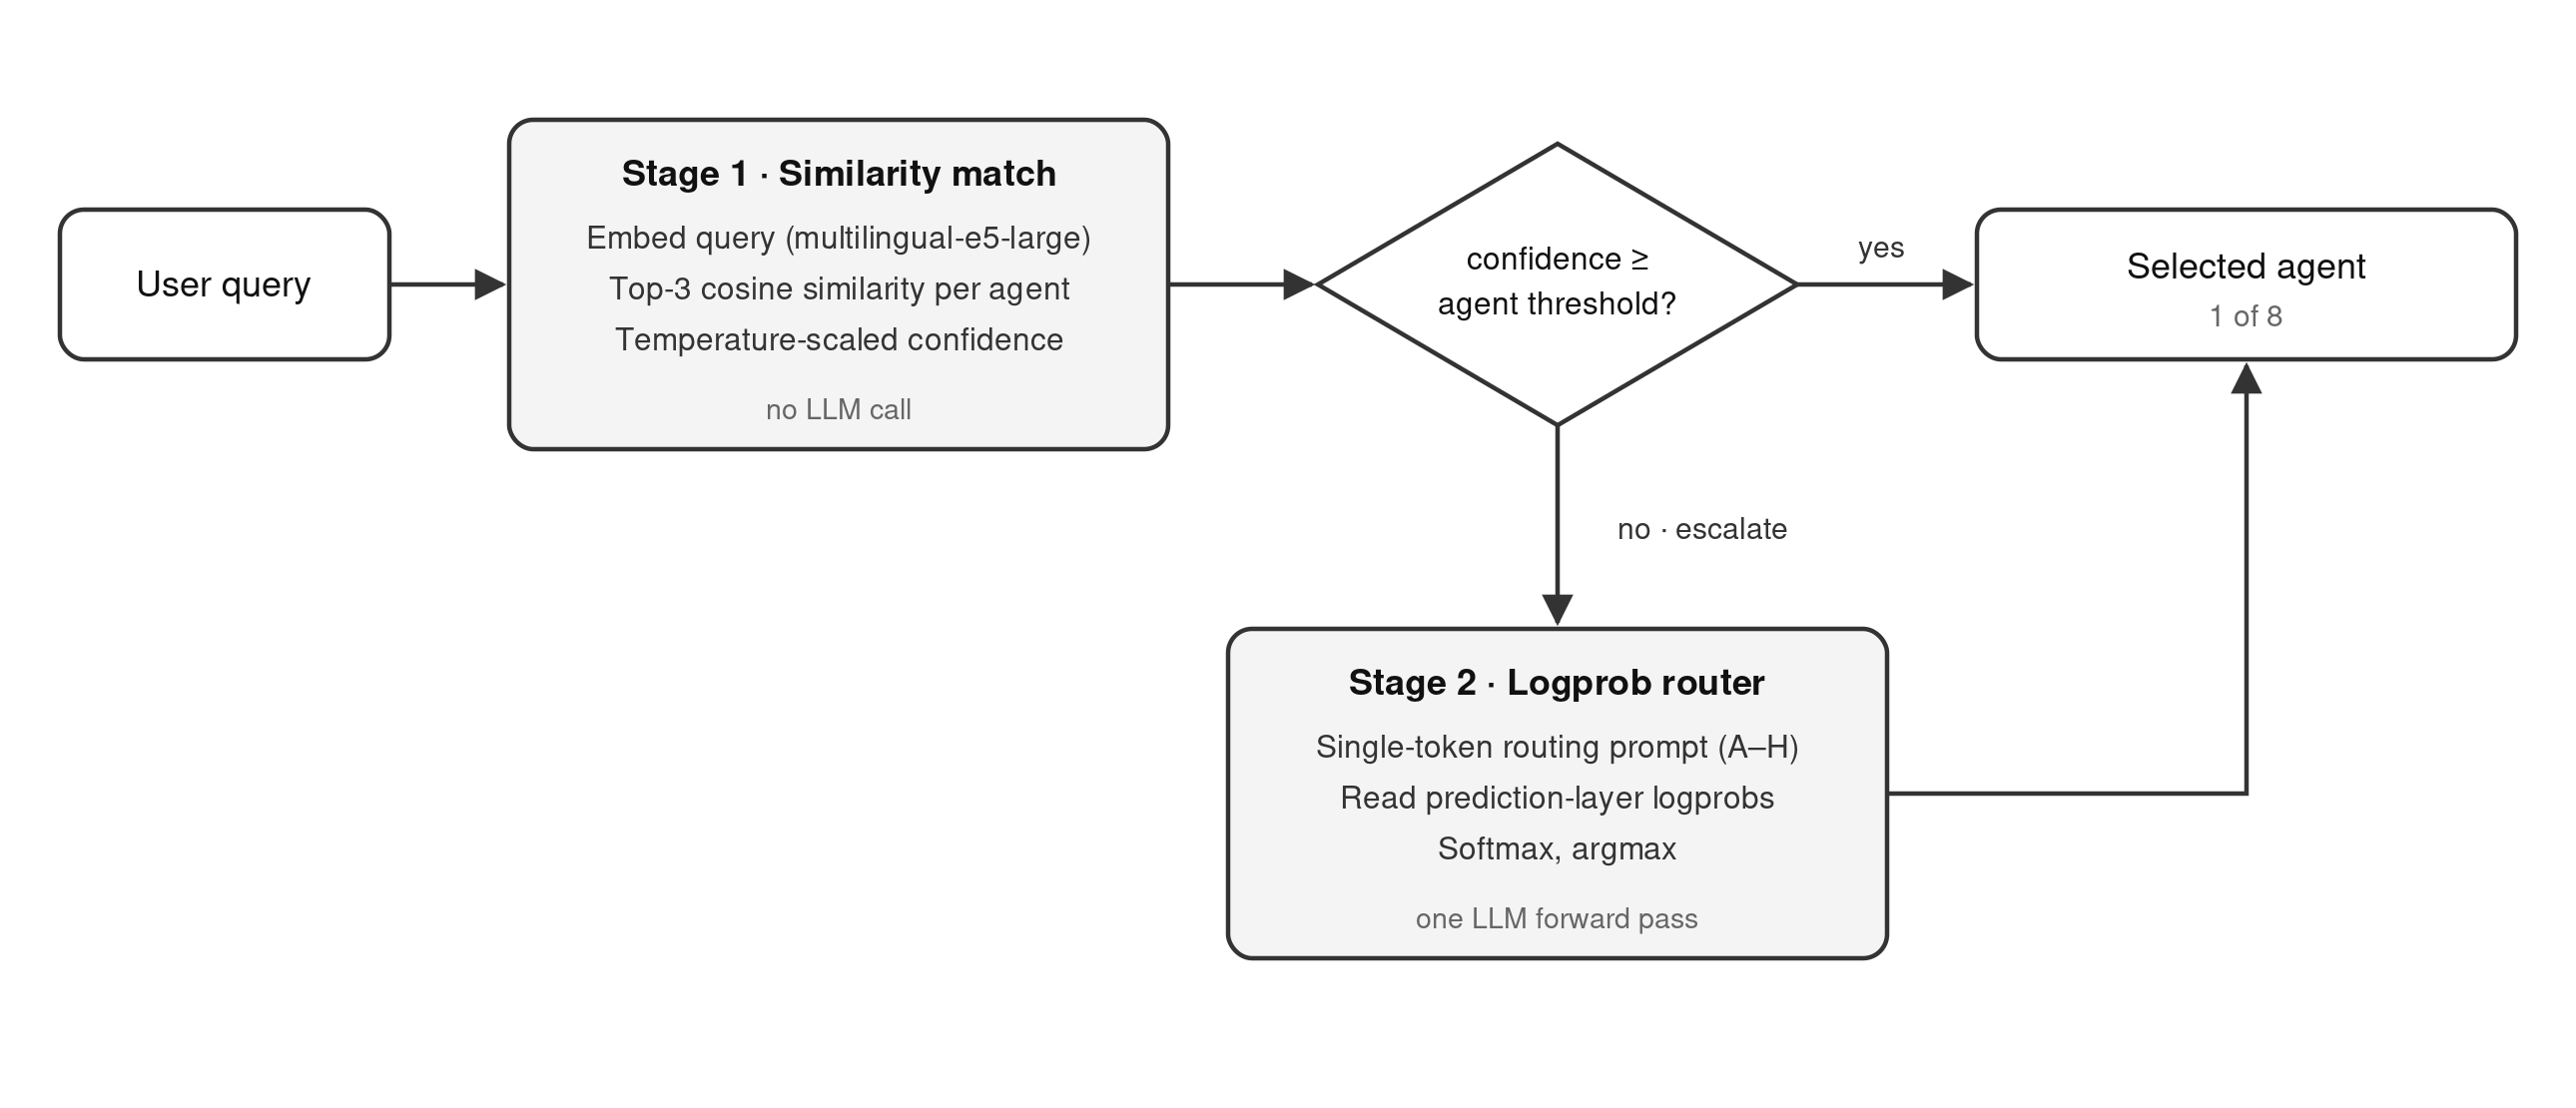
\includegraphics[width=1\linewidth,height=\textheight,keepaspectratio]{assets/router/fig-4-1-two-stage-pipeline.png}
\caption{Two-stage routing pipeline. Stage 1 resolves recognizable queries without an LLM call, Stage 2 deliberates over escalated cases (own illustration).}\label{fig:pipeline}
\end{figure}

\subsubsection{Stage 1, Routing by Semantic Similarity}\label{sec:router-stage1}

Stage 1 rests on a vector store of labeled reference queries, each stored with its embedding and agent label. The store is seeded from the golden dataset and grows through judge-confirmed production traces (\cref{sec:judge}). An incoming query is embedded with multilingual-e5-large, a self-hosted model producing 1024-dimensional vectors \autocite{wang2024}. Broker queries arrive in German and English, often mixed within one conversation, and the multilingual model maps both into one shared vector space, so a German query can match an English reference about the same task. Self-hosting keeps embedding cost independent of query volume and query content on our own infrastructure.

Each agent is scored by the mean cosine similarity between the query vector and its three closest reference queries. Our first design condensed every agent into a single centroid vector. This proved too coarse. An agent such as GeneralPurpose covers heterogeneous subtasks whose embeddings share no common center, and averaging them yields a representative vector that reflects none of them well. Scoring against individual reference queries preserves this local structure, so the instance-based variant replaced the centroid.

Raw cosine scores proved unsuitable as a decision signal. Embedding spaces are anisotropic, meaning the vectors concentrate in a narrow cone, which compresses all similarities into a tight band and makes absolute values hard to interpret \autocite{ethayarajh2019,steck2024}. All embeddings are therefore centered by subtracting the mean vector of the reference store and renormalizing, which spreads the similarity distribution. On top of that, we considered three variants of the decision signal. Variant A uses the raw margin between best and second-best agent score, Variant B the same margin on centered embeddings, and Variant C a temperature-scaled softmax over the per-agent scores, using the top-agent probability, with the temperature fitted on calibration data by minimizing negative log-likelihood \autocite{guo2017}. We selected Variant C on conceptual grounds rather than a measured accuracy difference. A probability between zero and one can be monitored directly, remains comparable across agents, and costs nothing mathematically, since temperature scaling provably cannot alter the agent ranking.

Whether Stage 1 may route directly is governed by calibrated thresholds. We fixed an error budget of five percent for directly routed queries and determined, per agent, the lowest confidence threshold at which the empirical error on held-out calibration data (1,000 queries, at least 50 per agent) stays within that budget. This follows conformal calibration, which converts a held-out sample into distribution-free error control \autocite{angelopoulos2023}. Thresholds are fitted per agent because score distributions differ substantially between agents. The fitted values range from 33.5 percent for GeneralPurpose to 94.2 percent for PlatformSupport. An agent falling below ten calibration samples reverts to a pooled global threshold. Because centering mean and score distribution shift as the store grows, thresholds are refitted periodically after judge-loop extensions (\cref{sec:judge}). \Cref{fig:risk-coverage} shows the resulting risk-coverage curve, with the deployed operating point at 96 percent coverage and 4.9 percent risk, inside the budget.

\begin{figure}
\centering
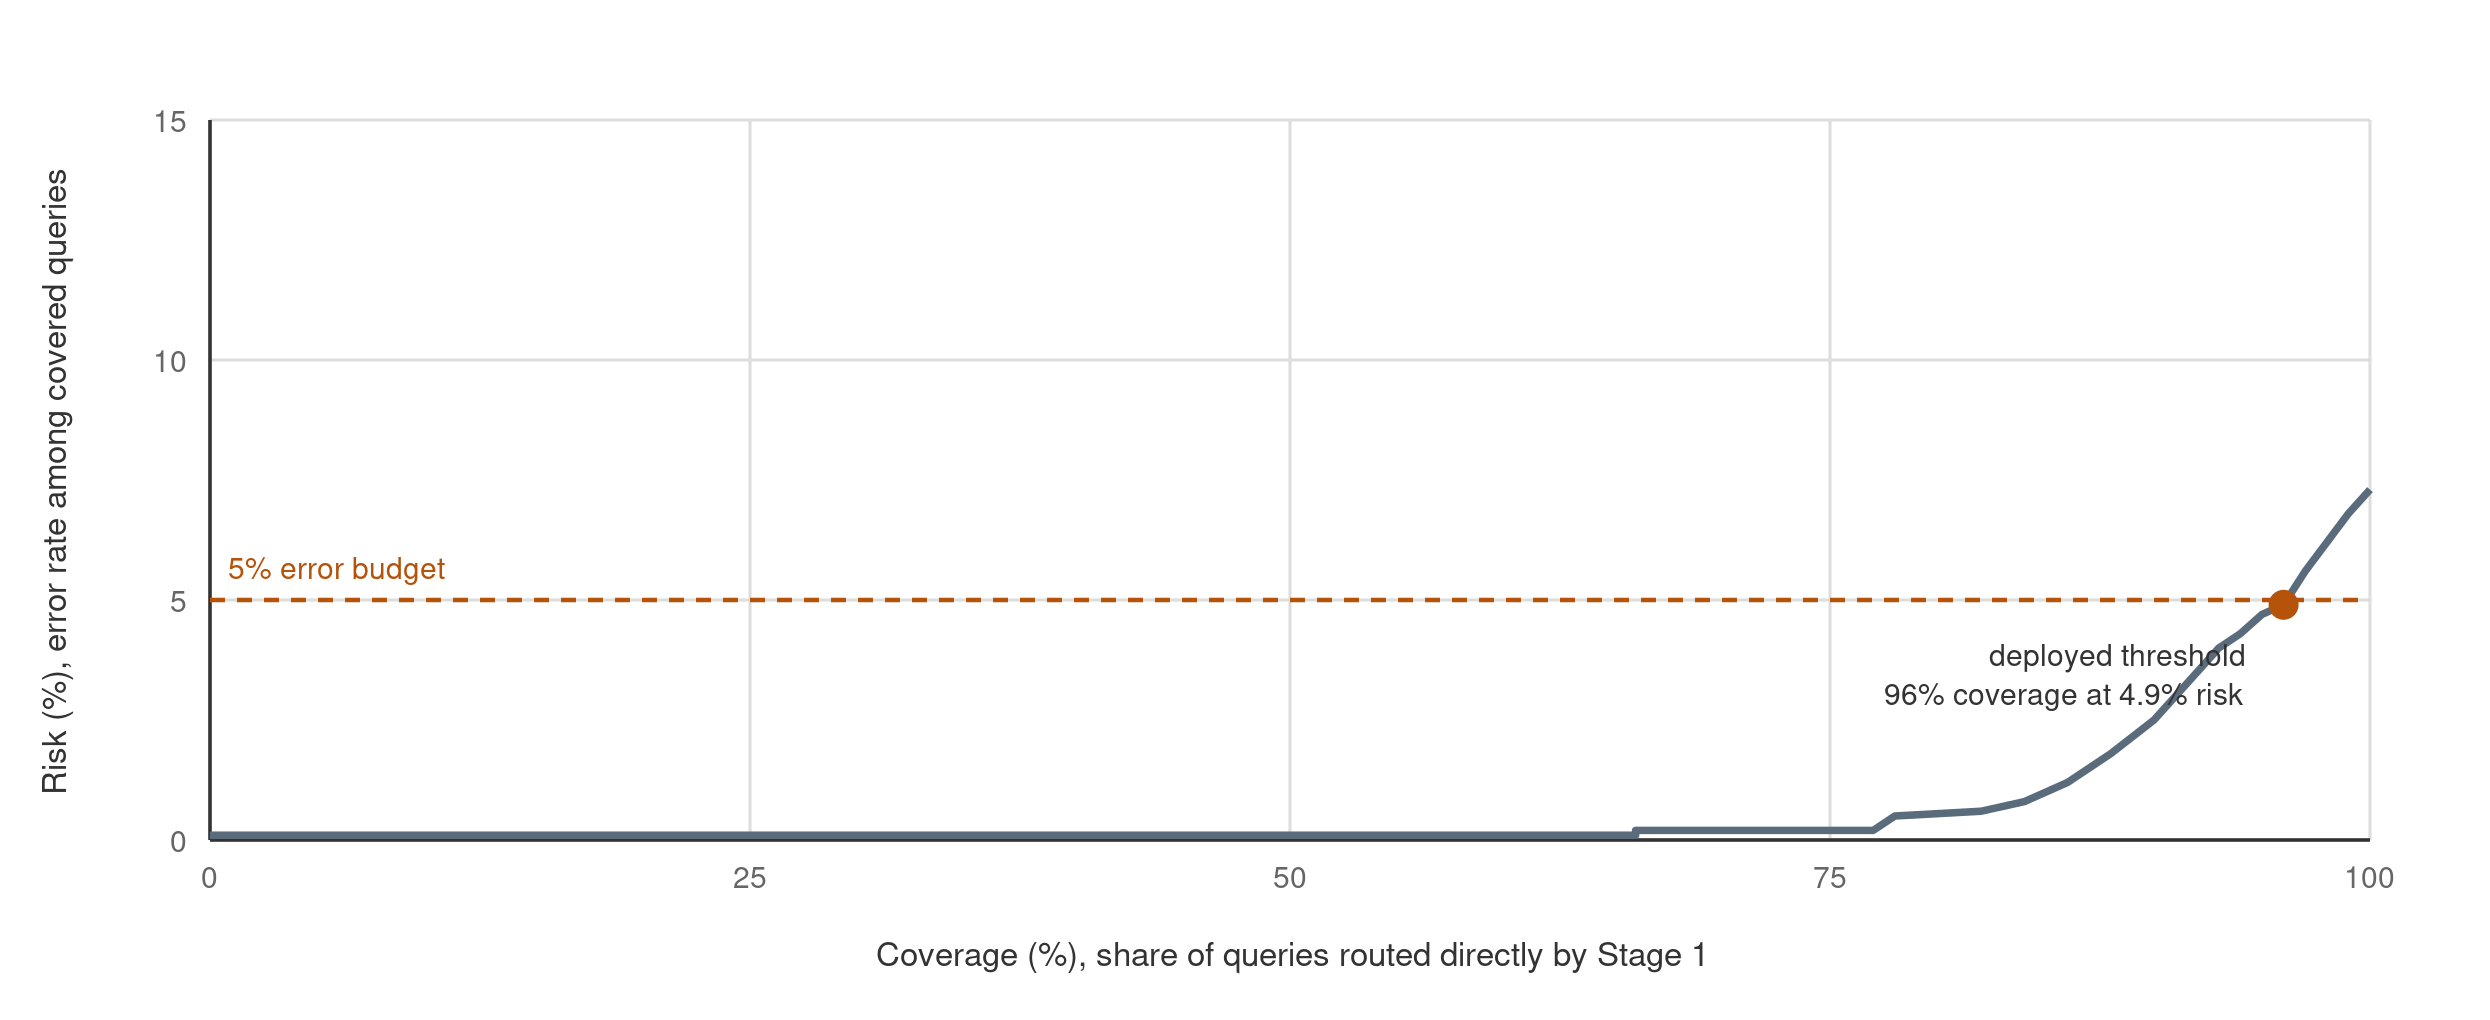
\includegraphics[width=1\linewidth,height=\textheight,keepaspectratio]{assets/router/fig-4-2-risk-coverage.png}
\caption{Risk-coverage curve of the calibrated Stage 1 router on held-out calibration data. The deployed operating point covers 96 percent of queries at 4.9 percent risk (own illustration).}\label{fig:risk-coverage}
\end{figure}

To protect the validity of this procedure, reference store and calibration set are disjoint, near-duplicates (similarity 0.99 or higher) are excluded as self-matches, and coverage and risk are estimated with five-fold cross-conformal validation rather than on the fitting data. A query that clears its agent's threshold is routed directly. Everything else escalates, which turns Stage 1 into a selective classifier that abstains whenever its confidence is insufficient \autocite{geifman2017}. In code, the decision reduces to two lines, all learned quantities loaded as configuration (\cref{fig:stage1-code}).

\begin{figure}
\centering
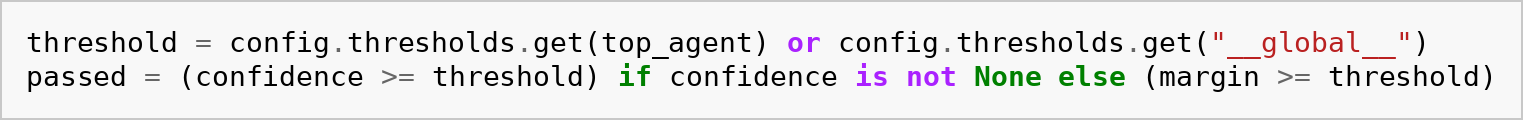
\includegraphics[width=1\linewidth,height=\textheight,keepaspectratio]{assets/router/fig-4-3-stage1-decision-rule.png}
\caption{Stage 1 decision rule, calibrated confidence against the per-agent threshold (\protect\texttt{router.py}).}\label{fig:stage1-code}
\end{figure}

\subsubsection{Stage 2, Routing by Log Probabilities}\label{sec:router-stage2}

Queries that Stage 1 abstains from escalate to a Gemma 4 E4B model, served locally through Ollama and dedicated to routing. The eight agents are encoded as fixed single-token identifiers, the letters A through H, and the routing prompt instructs the model to answer with exactly one of them. Instead of sampling that answer, we request the top log probabilities alongside the generated token and read the admissible route codes directly from the prediction layer. These are renormalized over the observed codes. A code missing from the returned candidates receives zero probability, a slight truncation bias we accept for simplicity. One forward pass thus yields a deterministic distribution over all eight agents, which matters for reproducible evaluation. Stage 2 always routes to its top candidate. As the final stage it has no abstention option, and its probabilities enter the decision uncalibrated, resting on the reliability that \textcite{kadavath2022} report for internal signals. The distribution is logged in full with every trace. Its runner-up later lets the judge compare the chosen agent against the strongest alternative (\cref{sec:judge}). The routing prompt is versioned so that the optimizer can improve it over time (\cref{sec:optimizer}), making it data rather than code, and the model sits behind a provider interface, so a different routing model requires a new provider class and no change to the dispatch logic.

The routing call generates exactly one token and asks the runtime for the log probabilities of the most likely tokens, from which the route codes are extracted and renormalized (\cref{fig:stage2-code}).

\begin{figure}
\centering
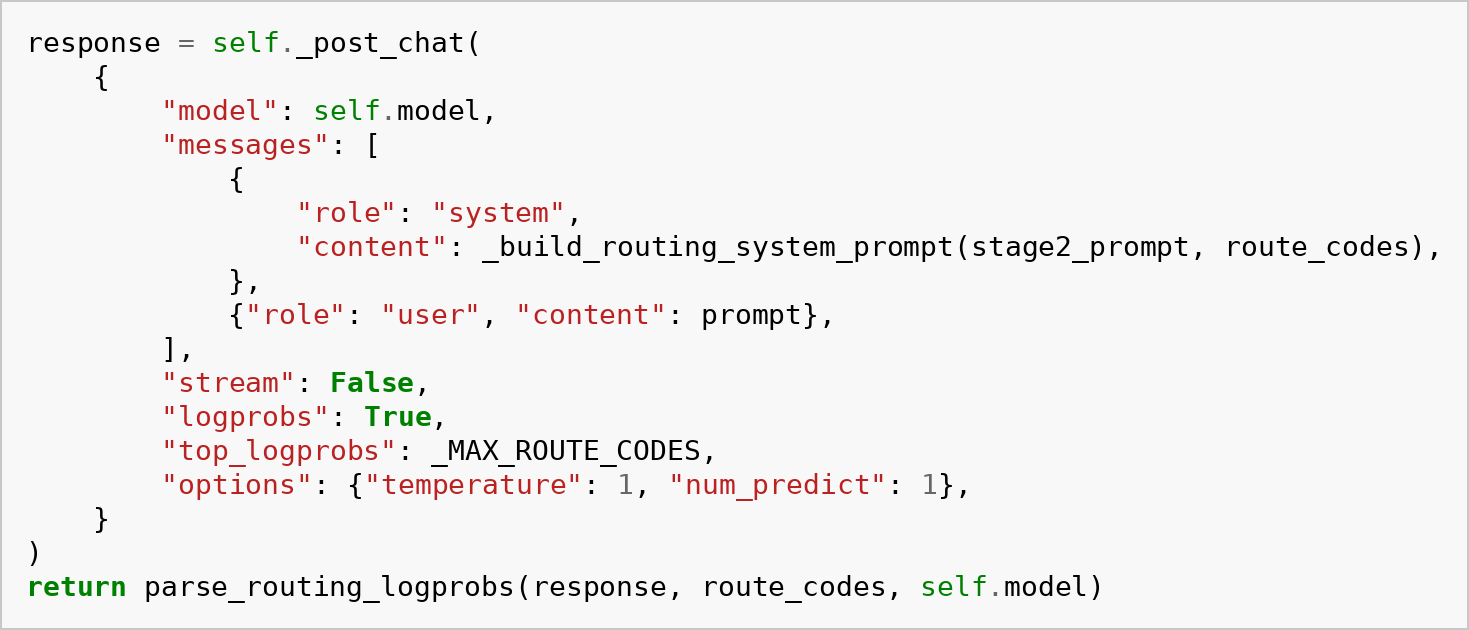
\includegraphics[width=0.9\linewidth,height=\textheight,keepaspectratio]{assets/router/fig-4-4-stage2-routing-call.png}
\caption{Stage 2 routing call, one generated token with token-level log probabilities (\protect\texttt{providers/ollama.py}, shortened for presentation).}\label{fig:stage2-code}
\end{figure}

\subsubsection{Integrated Workflow and Reflection}\label{sec:router-workflow}

At dispatch time the router loads the active configuration, embeds the query, and runs Stage 1. If the calibrated confidence clears the threshold, the selected agent answers immediately. Otherwise Stage 2 decides. Every trace records the path taken, both stages' scores, and all latencies (\cref{fig:dispatch-flow}).

\begin{figure}
\centering
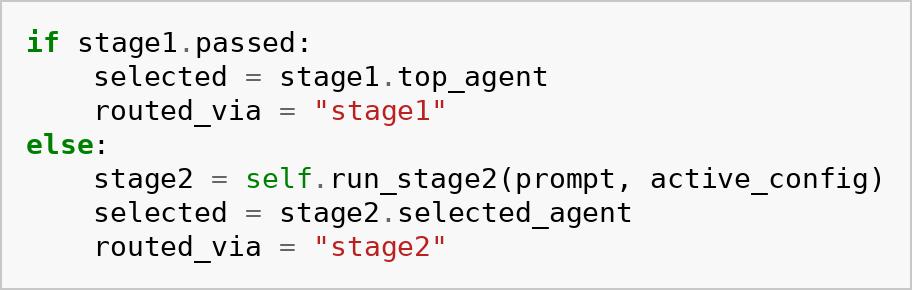
\includegraphics[width=0.75\linewidth,height=\textheight,keepaspectratio]{assets/router/fig-4-5-dispatch-flow.png}
\caption{Escalation logic in the dispatch flow (\protect\texttt{router.py}).}\label{fig:dispatch-flow}
\end{figure}

Compared to the initial system, which sent every query to an LLM and trusted its verbalized confidence, the two-stage design changes the operating characteristics in three ways. On the calibration distribution, 96 percent of queries never reach a language model, which cuts LLM calls and brings average latency down to embedding speed. Accuracy is nevertheless preserved, because Stage 1 only decides where its calibrated error stays within budget and hands every ambiguous case to the stronger mechanism. And the confidence signal is now read from model internals and calibrated on data instead of being stated by the model about itself. The system degrades gracefully, as Stage 1 still produces a ranked decision if the LLM runtime is unavailable. \Cref{sec:empirical-evaluation} quantifies these effects.

Some limitations remain. First, the calibrated thresholds guarantee the error budget only for the distribution of the calibration data, which is synthetic, so production drift requires recalibration. The long-run behavior of the judge loop that provides it was not observed within the project timeframe. Second, all findings rest on one embedding model and one routing model family, and the ranking of mechanisms could shift for models with differently calibrated logits. Third, the log-probability design presupposes a serving stack that exposes token-level probabilities, which restricts the choice of inference runtimes. Fourth, Stage 2 has no abstention option and routes on uncalibrated probabilities. A second selective layer, such as a clarifying question to the broker, remains future work.
